\subsection{Restriction and Prolongation operations}

Until this moment we have not talked about the grid size $N_x$ and $N_y$. To make things as simply as possible in this report, we only allow the grid size to be a power of two.

\begin{equation}
2^M = max(N_x, N_y)
\end{equation}

Before we break down the Multigrid algorithm itself, we need a method to go from a matrix $A^M$ with resolution $N_x,N_y$ to a lower resolution matrix $A^{M-1}$ with dimensions halfed in size, i.e $N_x/2,N_y/2$. In general, we need an operation that uses a matrix $A^{M-m}$ with dimensions $\frac{N_x}{2^m}$ as an input and produces a scaled matrix $A^{M-m-1}$. This operation is called restriction. In this report we will use bilinear interpolation for downscaling a matrix.

\begin{equation}
A^{M-n-1}_{i,j} = \frac{1}{4} ( A^{M-n}_{2i,2j} + A^{M-n}_{2i + 1,2j} + A^{M-n}_{2i + 1,2j +1 }  + A^{M-n}_{2i,2j + 1} )
\label{restricteq}
\end{equation}

Figure \ref {restrict} gives a numerical example of the restriction operation seen in Equation \ref{restricteq}

\begin{figure}[ht!]
\centering
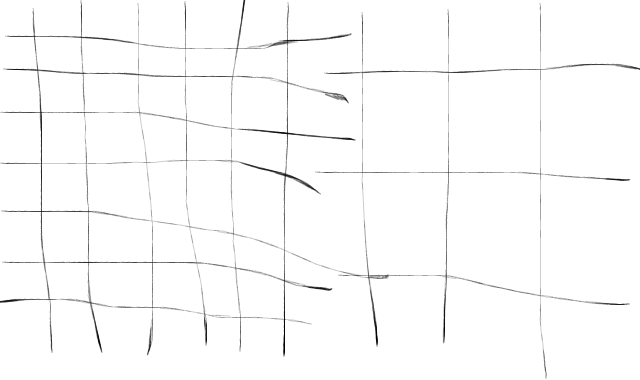
\includegraphics[width=120mm]{img/restrict.png}
\caption{A simple caption}
\label{restrict}
\end{figure}

To keep things simple, we also use bilinear interpolation in the prolongation operator where we do the opposite from restriction, i.e go from $A^{M-m}$ to $A^{M-m+1}$. Although using the same interpolation scheme, prolongation is a bit trickier to get right since the indices are not aligned up as perfect as in the restriction operator. Figure \ref {prolong} demonstrates why the indices are aligned slightly awkward.

\begin{figure}[ht!]
\centering
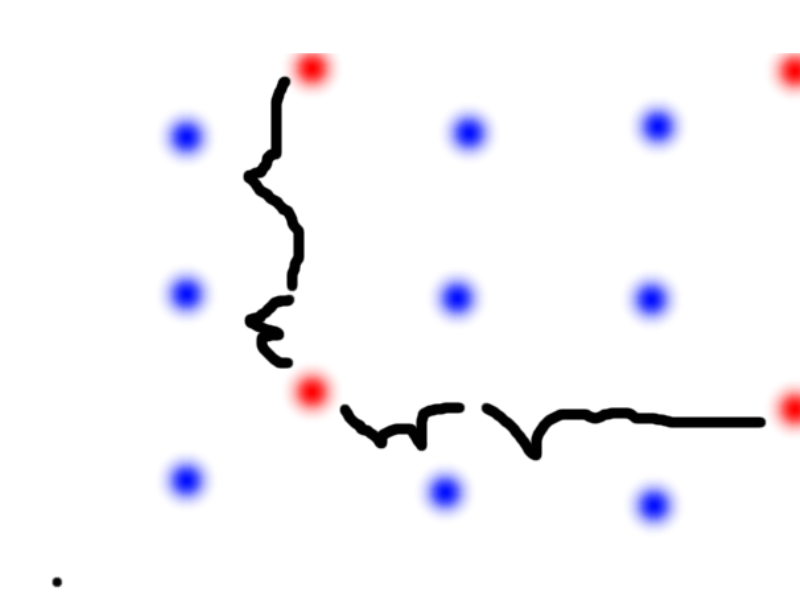
\includegraphics[width=80mm]{img/prolong.png}
\caption{A simple caption}
\label{prolong}
\end{figure}

To use the bilinear interpolation, we use the barycentric coordinates of each cell in $M-n$ compared to its neighboring cell in $M-n-1$ as can be seen in Figure \ref{prolong}. This gives us the following scheme for the prolongation operator:

\begin{equation}
\begin{split}
A^{M-n}_{2i,2j} &= \frac{1}{16} A^{M-n-1}_{i-1,j-1} +  \frac{3}{16} A^{M-n-1}_{i-1,j} +  \frac{3}{16} A^{M-n-1}_{i,j-1}+  \frac{9}{16} A^{M-n-1}_{i,j} \\ 
A^{M-n}_{2i + 1,2j} &= \frac{1}{16} A^{M-n-1}_{i+1,j-1} +  \frac{3}{16} A^{M-n-1}_{i,j-1} +  \frac{3}{16} A^{M-n-1}_{i+1,j}+  \frac{9}{16} A^{M-n-1}_{i,j} \\ 
A^{M-n}_{2i,2j+1} &= \frac{1}{16} A^{M-n-1}_{i-1,j+1} +  \frac{3}{16} A^{M-n-1}_{i-1,j} +  \frac{3}{16} A^{M-n-1}_{i,j+1}+  \frac{9}{16} A^{M-n-1}_{i,j} \\ 
A^{M-n}_{2i+1,2j+1} &= \frac{1}{16} A^{M-n-1}_{i+1,j+1} +  \frac{3}{16} A^{M-n-1}_{i+1,j} +  \frac{3}{16} A^{M-n-1}_{i,j+1}+  \frac{9}{16} A^{M-n-1}_{i,j} \\ 
\end{split}
\label{prolongeq}
\end{equation}

Equation \ref{prolongeq} only works if the updated cells are not on the boundary and has four neighboring cells in the lower dimension grid. If the cell is on the boundary, we use simple linear interpolation between the two cells in $A^{M-n-1}$ with weights $0.75$ and $0.25$. Before we move on to the Multigrid algorithm, there one last special case. At the four corners, we use the same value as the corners of the lower dimension grid since there is nothing nearby to interpolate from.
